%laden der Präambel mit Latexbefehlen/-klassen
% !TeX encoding = UTF-8

\documentclass[a0paper,landscape]{baposter}
\usepackage[english]{babel}
\usepackage[utf8]{inputenc}
%\usepackage{arev}
%\usepackage[T1]{fontenc}

\usepackage{marvosym}
\usepackage{pifont}
\usepackage{setspace}

\usepackage{makecell}

%for mathematical symbols
\usepackage{amsmath}
\usepackage{amsxtra}
\usepackage{eurosym}
\usepackage{siunitx}  
\sisetup{locale=DE}
\usepackage[version=4]{mhchem}

%Typography
\usepackage[auto]{microtype}

\usepackage{booktabs}
\usepackage{multirow}
\usepackage{paralist}

\usepackage[
backend=biber,
style=nature,
citestyle=numeric-comp,
sorting=none,
maxbibnames=1,
firstinits=true
]{biblatex}
%\usepackage{natbib}

\bibliography{biblio/refs,biblio/bibtemp}
\setlength\bibitemsep{2.5pt}

%colors
\definecolor{standardfontcolor}{RGB}{0,0,0} 
\definecolor{bordercol}{RGB}{113,113,113}
\definecolor{headercol1}{RGB}{255,255,255}
\definecolor{headercol2}{RGB}{113,113,113}
\definecolor{headerfontcol}{RGB}{0,0,0}
\definecolor{boxcolor}{RGB}{255,255,255}


\begin{document}
	\typeout{Poster rendering started}
	
\background{
	\begin{tikzpicture}[remember picture,overlay]%
	\draw (current page.north west)+(-2em,2em) node[anchor=north west]
	{\includegraphics[height=1.1\textheight]{figures/background}};
	\end{tikzpicture}
}

\color{standardfontcolor}

\begin{poster}{
		grid=false,
		columns=3,
		%colspacing=length
		headerheight=0.125\textheight,
		eyecatcher=false,
        borderColor=bordercol,
		headerColorOne=headercol1,
		headerColorTwo=headercol2,
		headerFontColor=headerfontcol,
		% Only simple background color used, no shading, so boxColorTwo isn't necessary
		boxColorOne=boxcolor,
		headershape=roundedright,
		headerfont=\sffamily\bfseries\Large,
		textborder=rectangle,
		headerborder=open,
		boxshade=plain,
		background=none
%		background=user
	}
	%%% Eye Cacther %%%%%%%%%%%%%%%%%%%%%%%%%%%%%%%%%%%%%%%%%%%%%%%%%%%%%%%%%%%%%%%
	{
		Eye Catcher, empty if option eyecatcher=false - unused
	}
%----------------------------------------------------------------------------------------
%	TITLE AND AUTHOR NAME
%----------------------------------------------------------------------------------------
%
{
	\textsf %Sans Serif
	{\vskip 2.0cm Exploring complex normal faulting systems \\ through physics-based dynamic modeling.}
}
{\sf\vspace{-0.1em}\\
	{\textbf{H.-S. S\'anchez-Reyes$^1$}, O. Scotti$^2$, S. Hok$^2$, A.-A. Gabriel$^3$ and T. Taufiqurrahman$^3$}
	\vspace{0.6em}\\
	\normalsize{$^1$Institut des Sciences de la Terre, IRD-UGA, BP 53, 38041 Grenoble Cedex 9, France \vspace{0.1em}\\
	$^2$Bureau d’Évaluation des Risques Sismiques pour la Sûreté des Installations, IRSN, 92260 Fontenay-aux-Roses, France
	\vspace{0.1em}\\
	$^3$Department of Earth and Environmental Sciences, Ludwig-Maximilians-Universitat, 80333 Munchen, Germany	 	
	} \\ \\ \\ \\ \\ 
}
% University/lab logo
{ \begin{minipage}{2cm}
  \vskip -0.2cm \hskip -5.2cm 
\includegraphics[width=7.1cm]{../../logos/logo_poster_2022.png} \\
 \end{minipage}
 }

 

\headerbox{{\bf 1.} Introduction}{name=intro,column=0,row=0,span=1}{

\vskip -0.5cm\begin{minipage}{0.5\linewidth}
\vskip -0cm 
 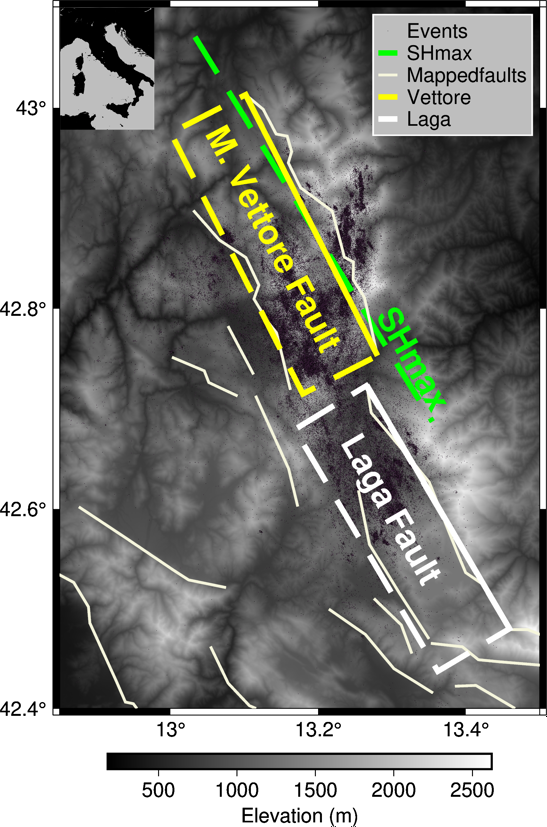
\includegraphics[width=1\linewidth]{images/Map_Italy}
\end{minipage}
\begin{minipage}{0.48\linewidth}
 \vskip 0.6cm {\small {\bf Geological context:}}
 \vskip 0.3cm
 {\small
 \begin{spacing}{1.0} 
 The Apennine seismic belt \\
 in Italy is an extensional\\
 province characterized by \\
 multi-fault normal-faulting\\
 seismic activity. Earthqua-\\
 kes and/or seismic sequen-\\
 ces ocurring across multi-\\
 fault segments during a \\
 single event (e.g. 1980 \\
 Ms 6.9 Irpinia Bernard \&\\
 Zollo (1989)) or sequences\\
 spanning a period of days \\
 (e.g. 2009 Mw 6.1 L’Aquila \\
 Valoroso et al (2013)) to
\end{spacing}
 }
\end{minipage}
\vskip -0.3cm{\small  months (e.g. 2016 Amatrice-Visso-Norcia Improta et al.\\ (2019)), are controlled by the physical complexities of \\
the active normal fault system. Understanding rupture \\
propagation across step-overs, breaking multiple fault\\
segments during a single earthquake, is crucial to enhan-\\
ce the current SHA Bai and Ampuero (2017).} \\ \nocite{Bai_2017_ESD}
\vskip -0.2cm
   \begin{tikzpicture}[%
    auto,
    block/.style={
      rectangle,
      draw=red!200,
      thick,
      fill=none,
      text width=\textwidth,
      align=justify,
      rounded corners,
      minimum height=4em
    },
    block1/.style={
      rectangle,
      draw=black,
      thick,
      fill=red!20,
      text width=\textwidth,
      align=center,
      rounded corners,
      minimum height=4em
    },
    line/.style={
      draw,thick,
      -latex',
      shorten >=4pt
    },
    cloud/.style={
      draw=red,
      thick,
      ellipse,
      fill=red!20,
      minimum height=4em
    }
  ]
    \draw (2.5,-2) node[block] (C) {
    \bf \color{red} \small Goal: Explore dynamic rupture parameters to better understand the physical condition promoting rupture jumps in normal faulting systems};     

  \end{tikzpicture} \vskip -0.2cm
}


\headerbox{{\bf 2.} Geometry-Settings}{name=geo,column=0,row=1,span=1,below=intro}{

\centering 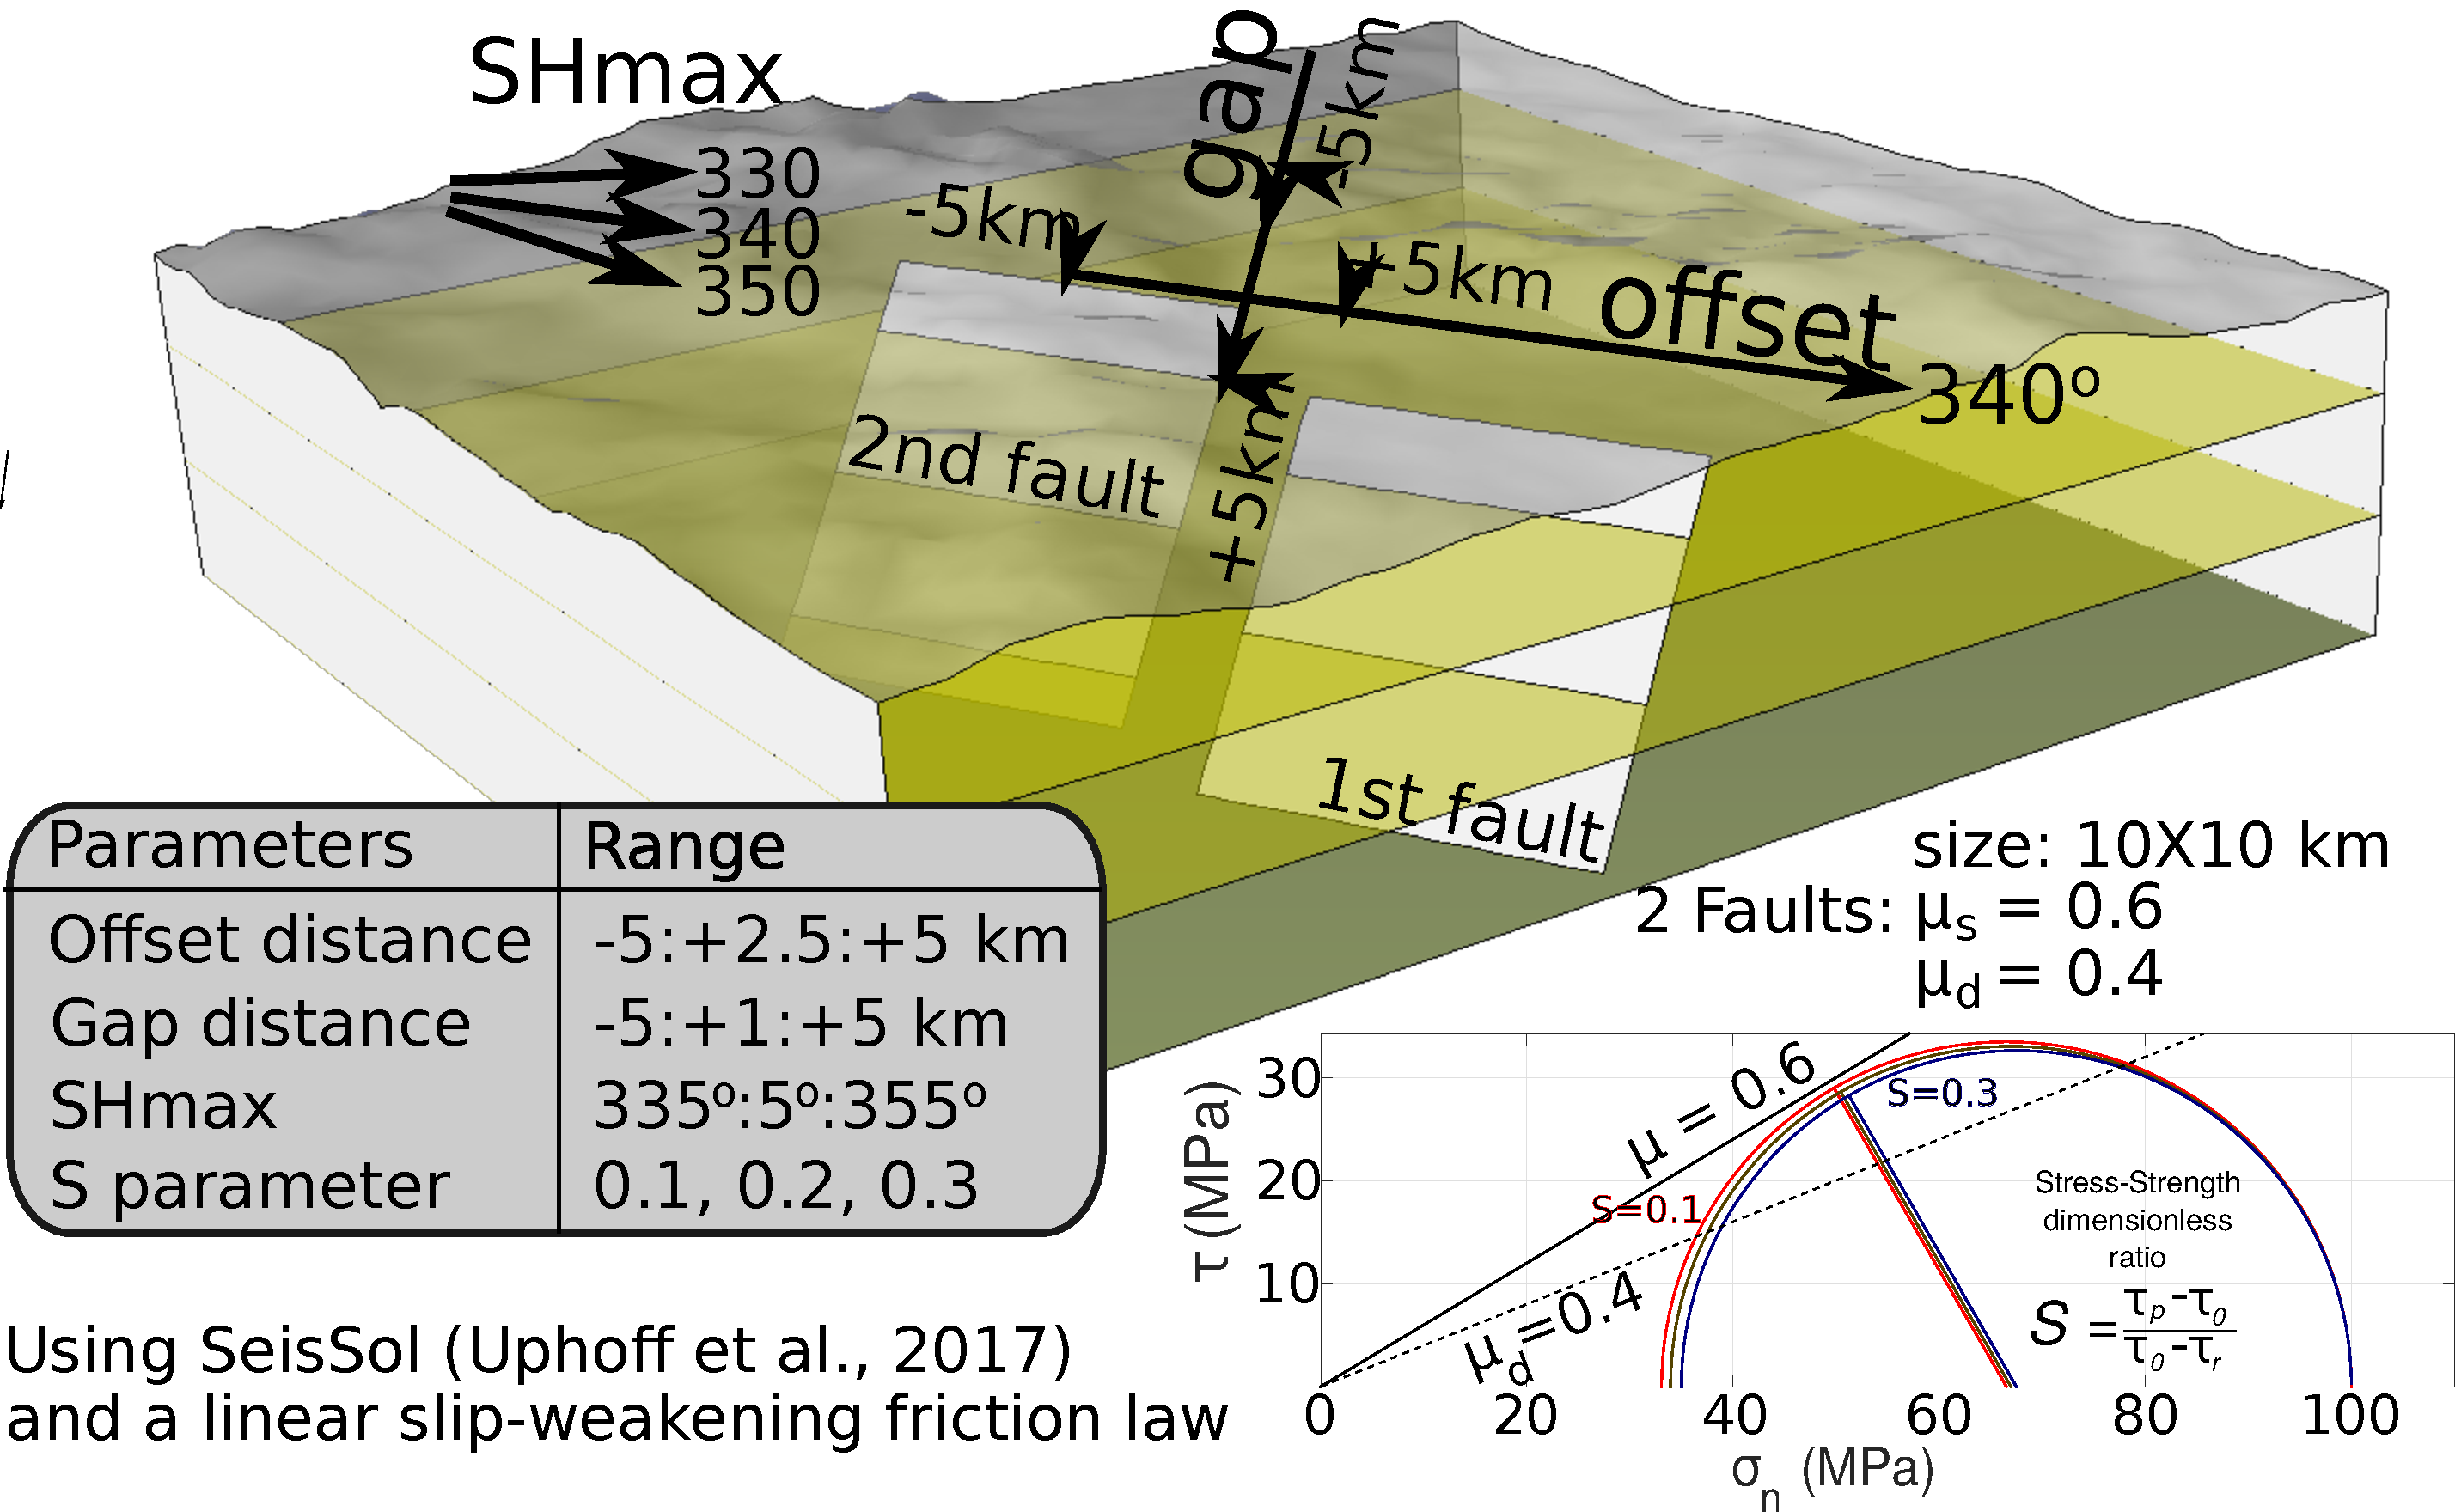
\includegraphics[width=1\linewidth]{images/model.pdf}
\vskip 0.3cm
%\begin{center}
% 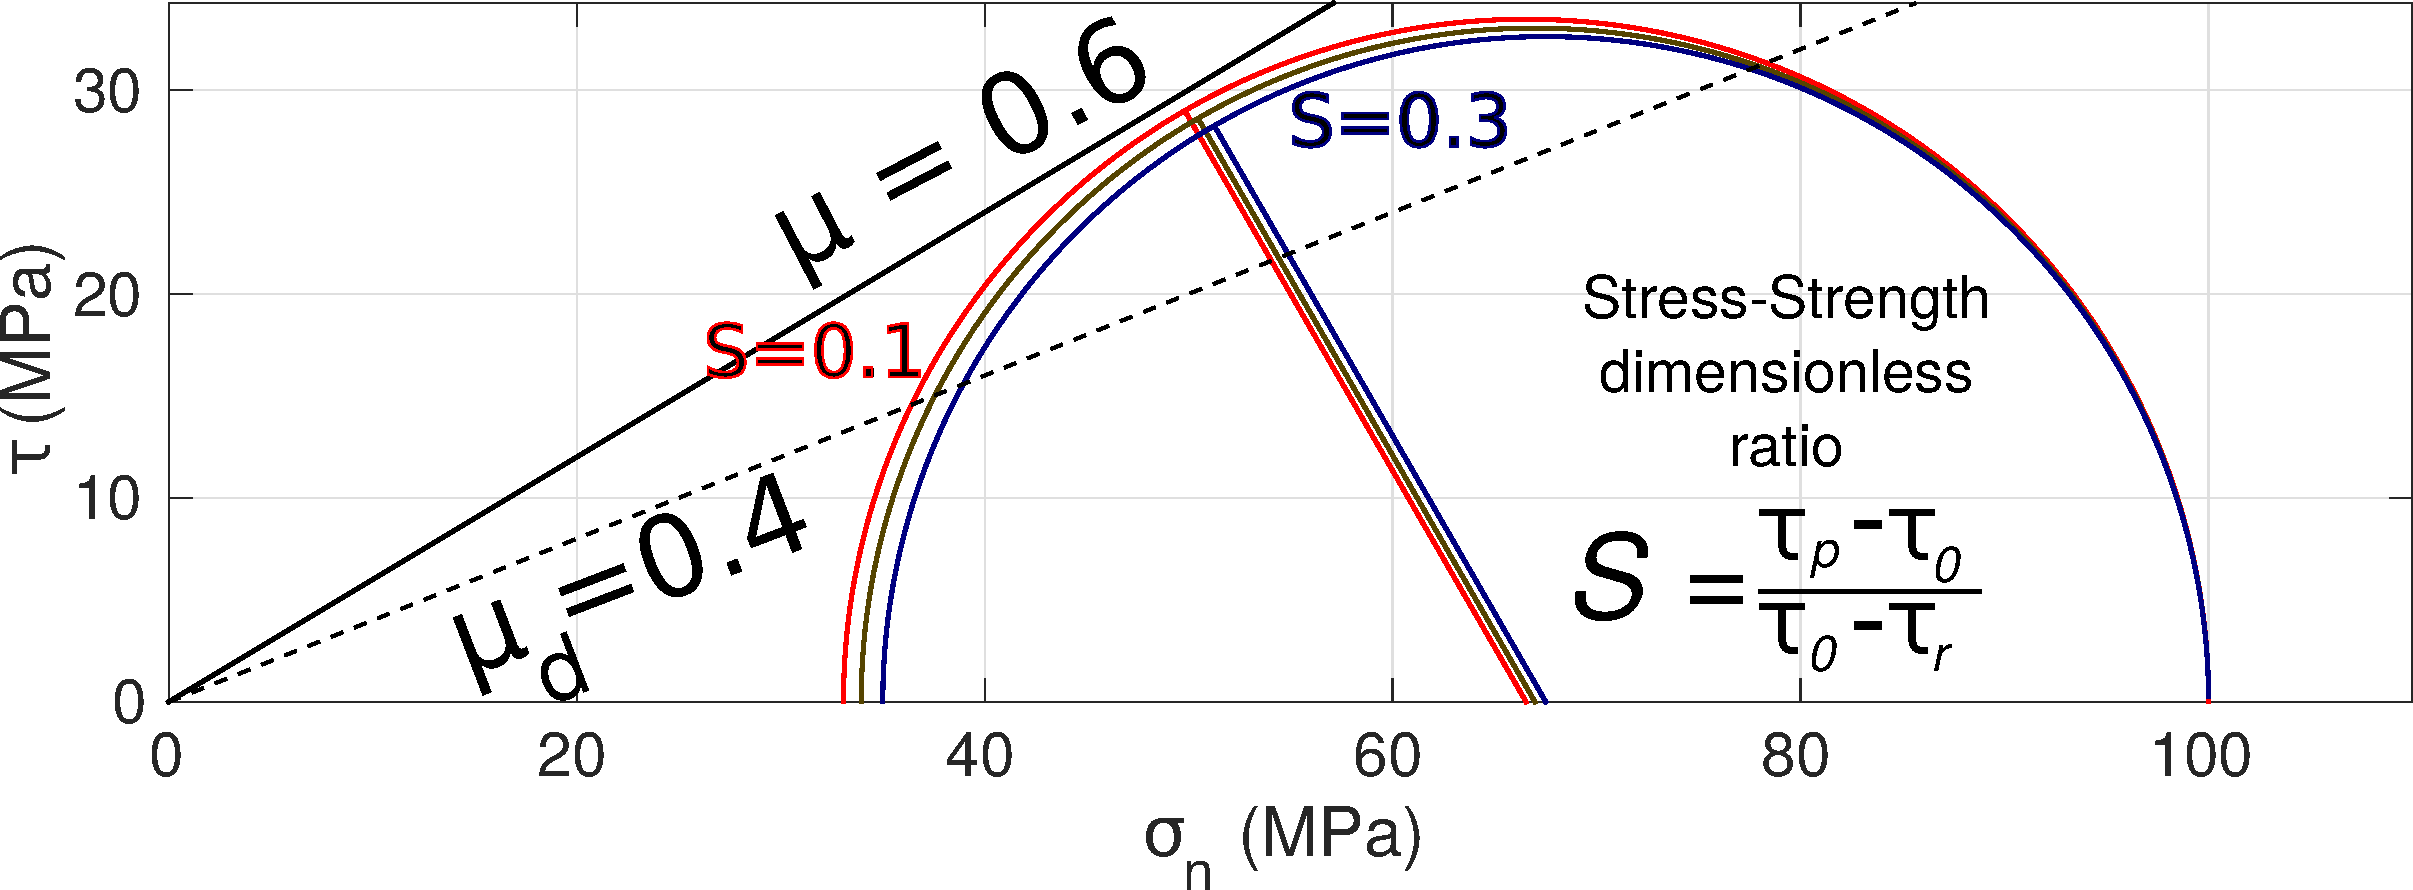
\includegraphics[width=0.75\linewidth]{images/MC_circle_new.pdf} 
%\end{center}
}



\headerbox{{\bf 3.} Simulation-Results}{name=summary,column=0,row=2,span=1,below=geo}{

\begin{minipage}{1\linewidth}
\vskip -0cm \centering 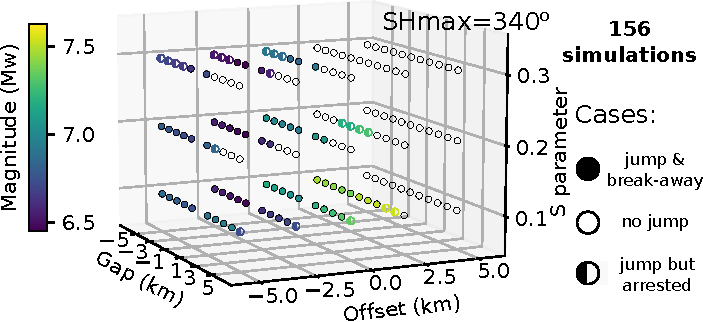
\includegraphics[width=1\linewidth]{images/tests_shmax340.pdf}
\end{minipage} 
\vskip 0.25cm
Some cases did not break the second fault, due to\\
the distance between faults (large offsets and gaps),\\ effect enhanced by prestress state (large $S$, small\\ stress). Overlap (Offset<0) promotes the jump.\\
\vskip -0.25cm
\textbf{Hanging/foot wall asymmetry:} \\
\vskip -0.25cm
Regarding the second fault location with
respect to \\ 
the main fault (hanging or foot wall), when the se-
\\cond fault is on the hanging wall (Gap$<$0), the 
dy-\\
namically triggered rupture is more likely to be\\
triggered and sustainable.\\ 
\vskip -0.25cm
\textbf{Stress shadow:} \\
\vskip -0.25cm
The final energy released (M$_w$) increases/decreases\\ according to the distance between faults (offset \& \\
gap). Although the overlap increases the triggering \\
effect, the stress shadow due to the fault proximity\\
inhibits a large stress drop on the 2nd fault.
}


\headerbox{{\bf 4.} Jump ? How ? When ? Why ?}{name=snaps,column=1,row=0,span=2}{

\begin{minipage}{0.667\linewidth}
\vskip -0.0cm \centering {\bf Fault not fixed ($\mu_s=0.6$) \qquad (dynamic analysis)} \vskip 0.1cm
 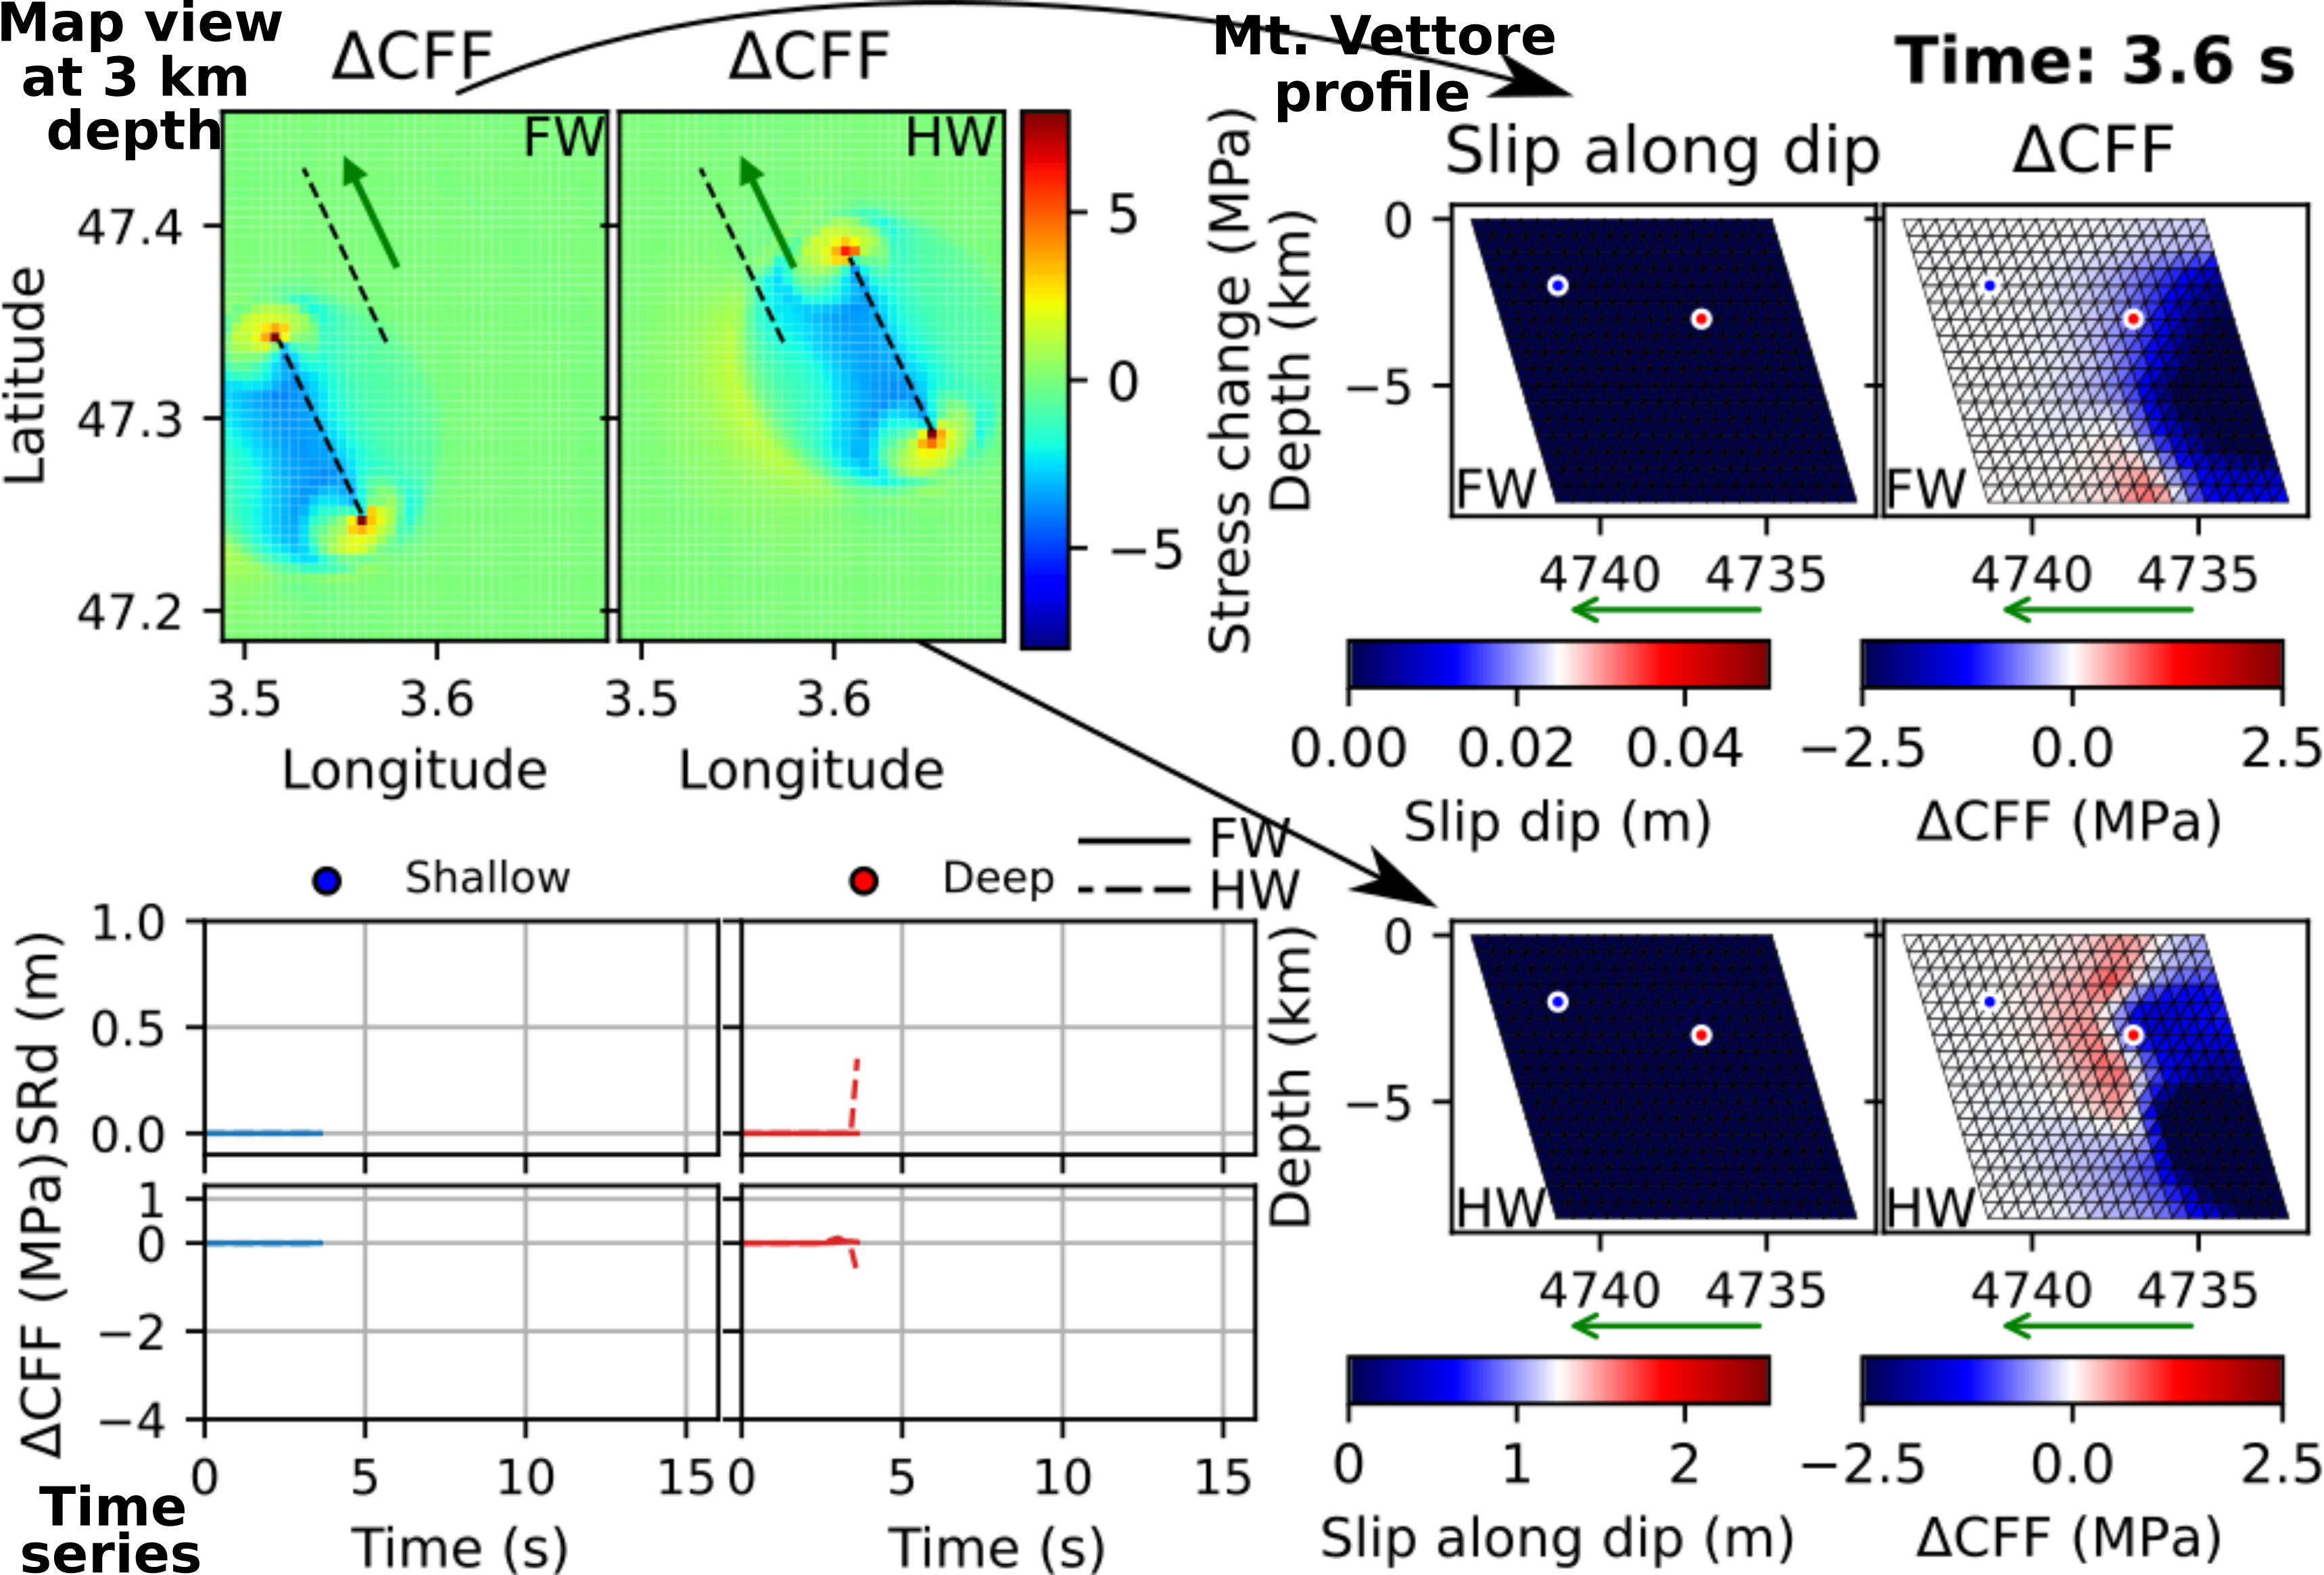
\includegraphics[width=0.92\linewidth]{images/horizontal_delta_00018_nofix.png}
\vskip 0.2cm
\hrule height 0.05cm
\vskip 0.2cm
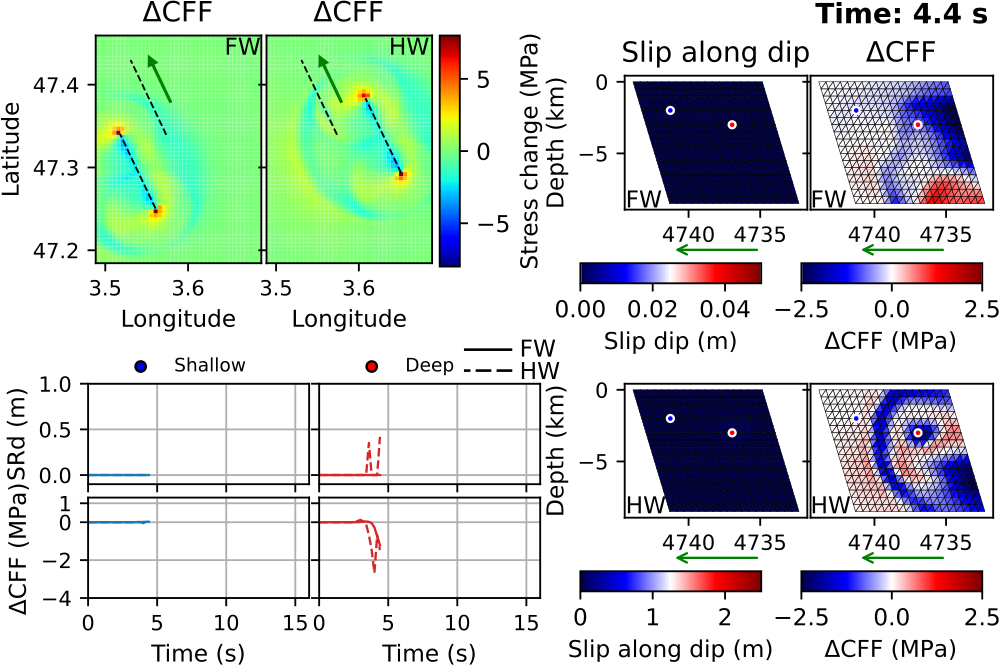
\includegraphics[width=0.92\linewidth]{images/horizontal_delta_00022_nofix.png} \\
\vskip 0.2cm
\hrule height 0.05cm
\vskip 0.2cm
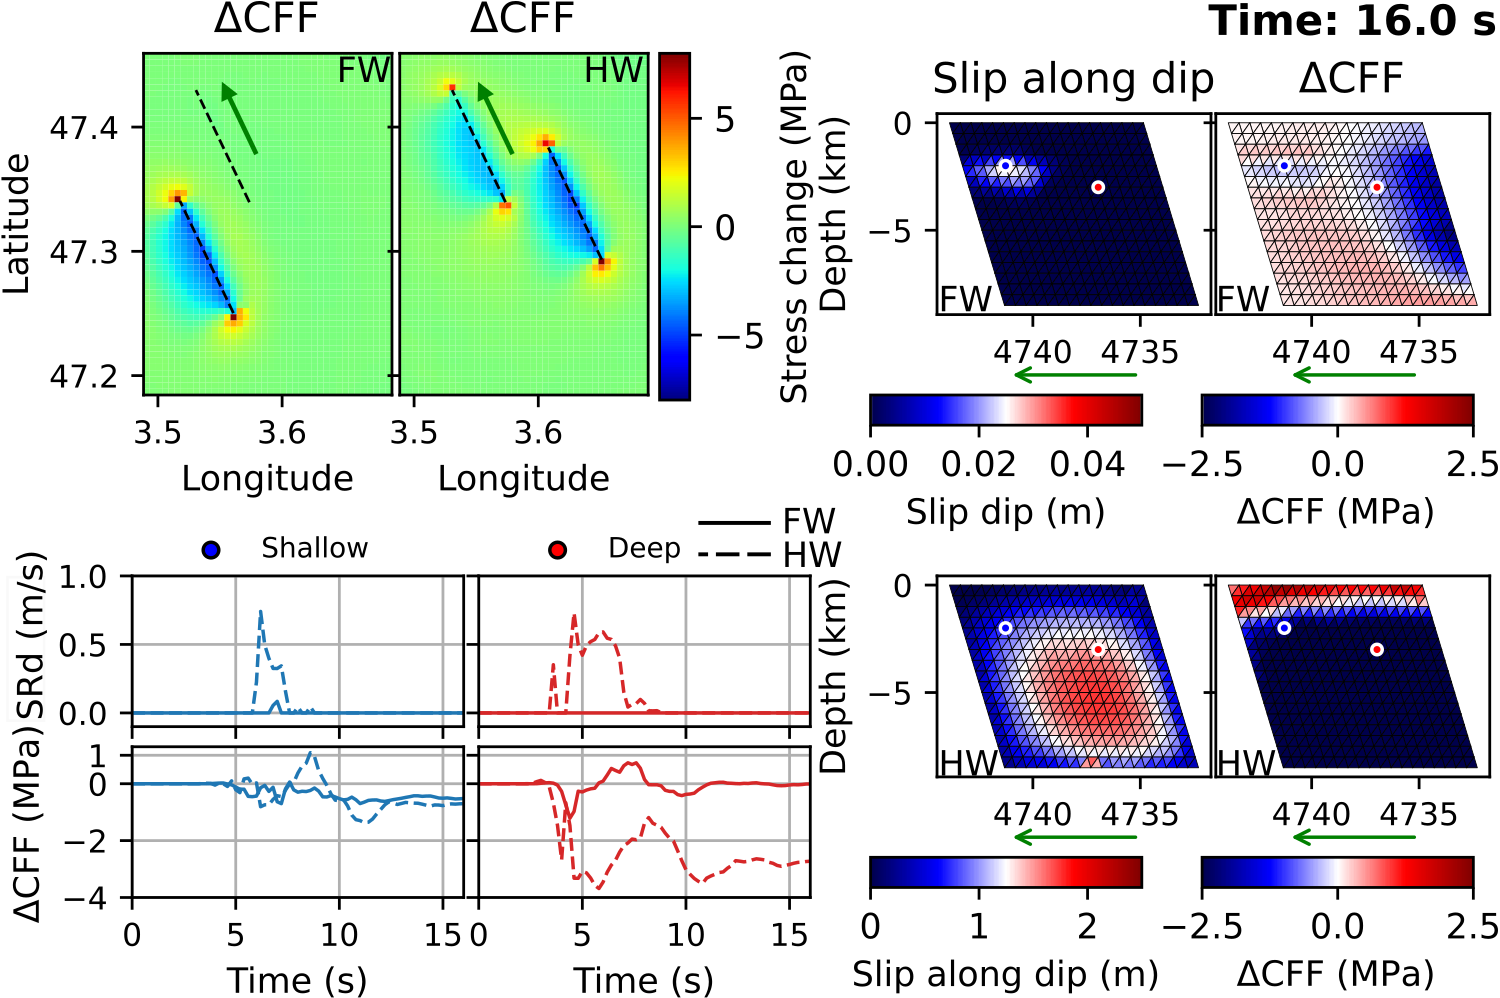
\includegraphics[width=0.92\linewidth]{images/horizontal_delta_00080_nofix.png} 
\end{minipage} \vrule width 0.05cm
\begin{minipage}{0.32\linewidth}
\vskip 0.1cm
\centering Slip rate snapshots \\
fault not fixed \& \\ break-away behavior \\
\vskip 0.15cm
\centering 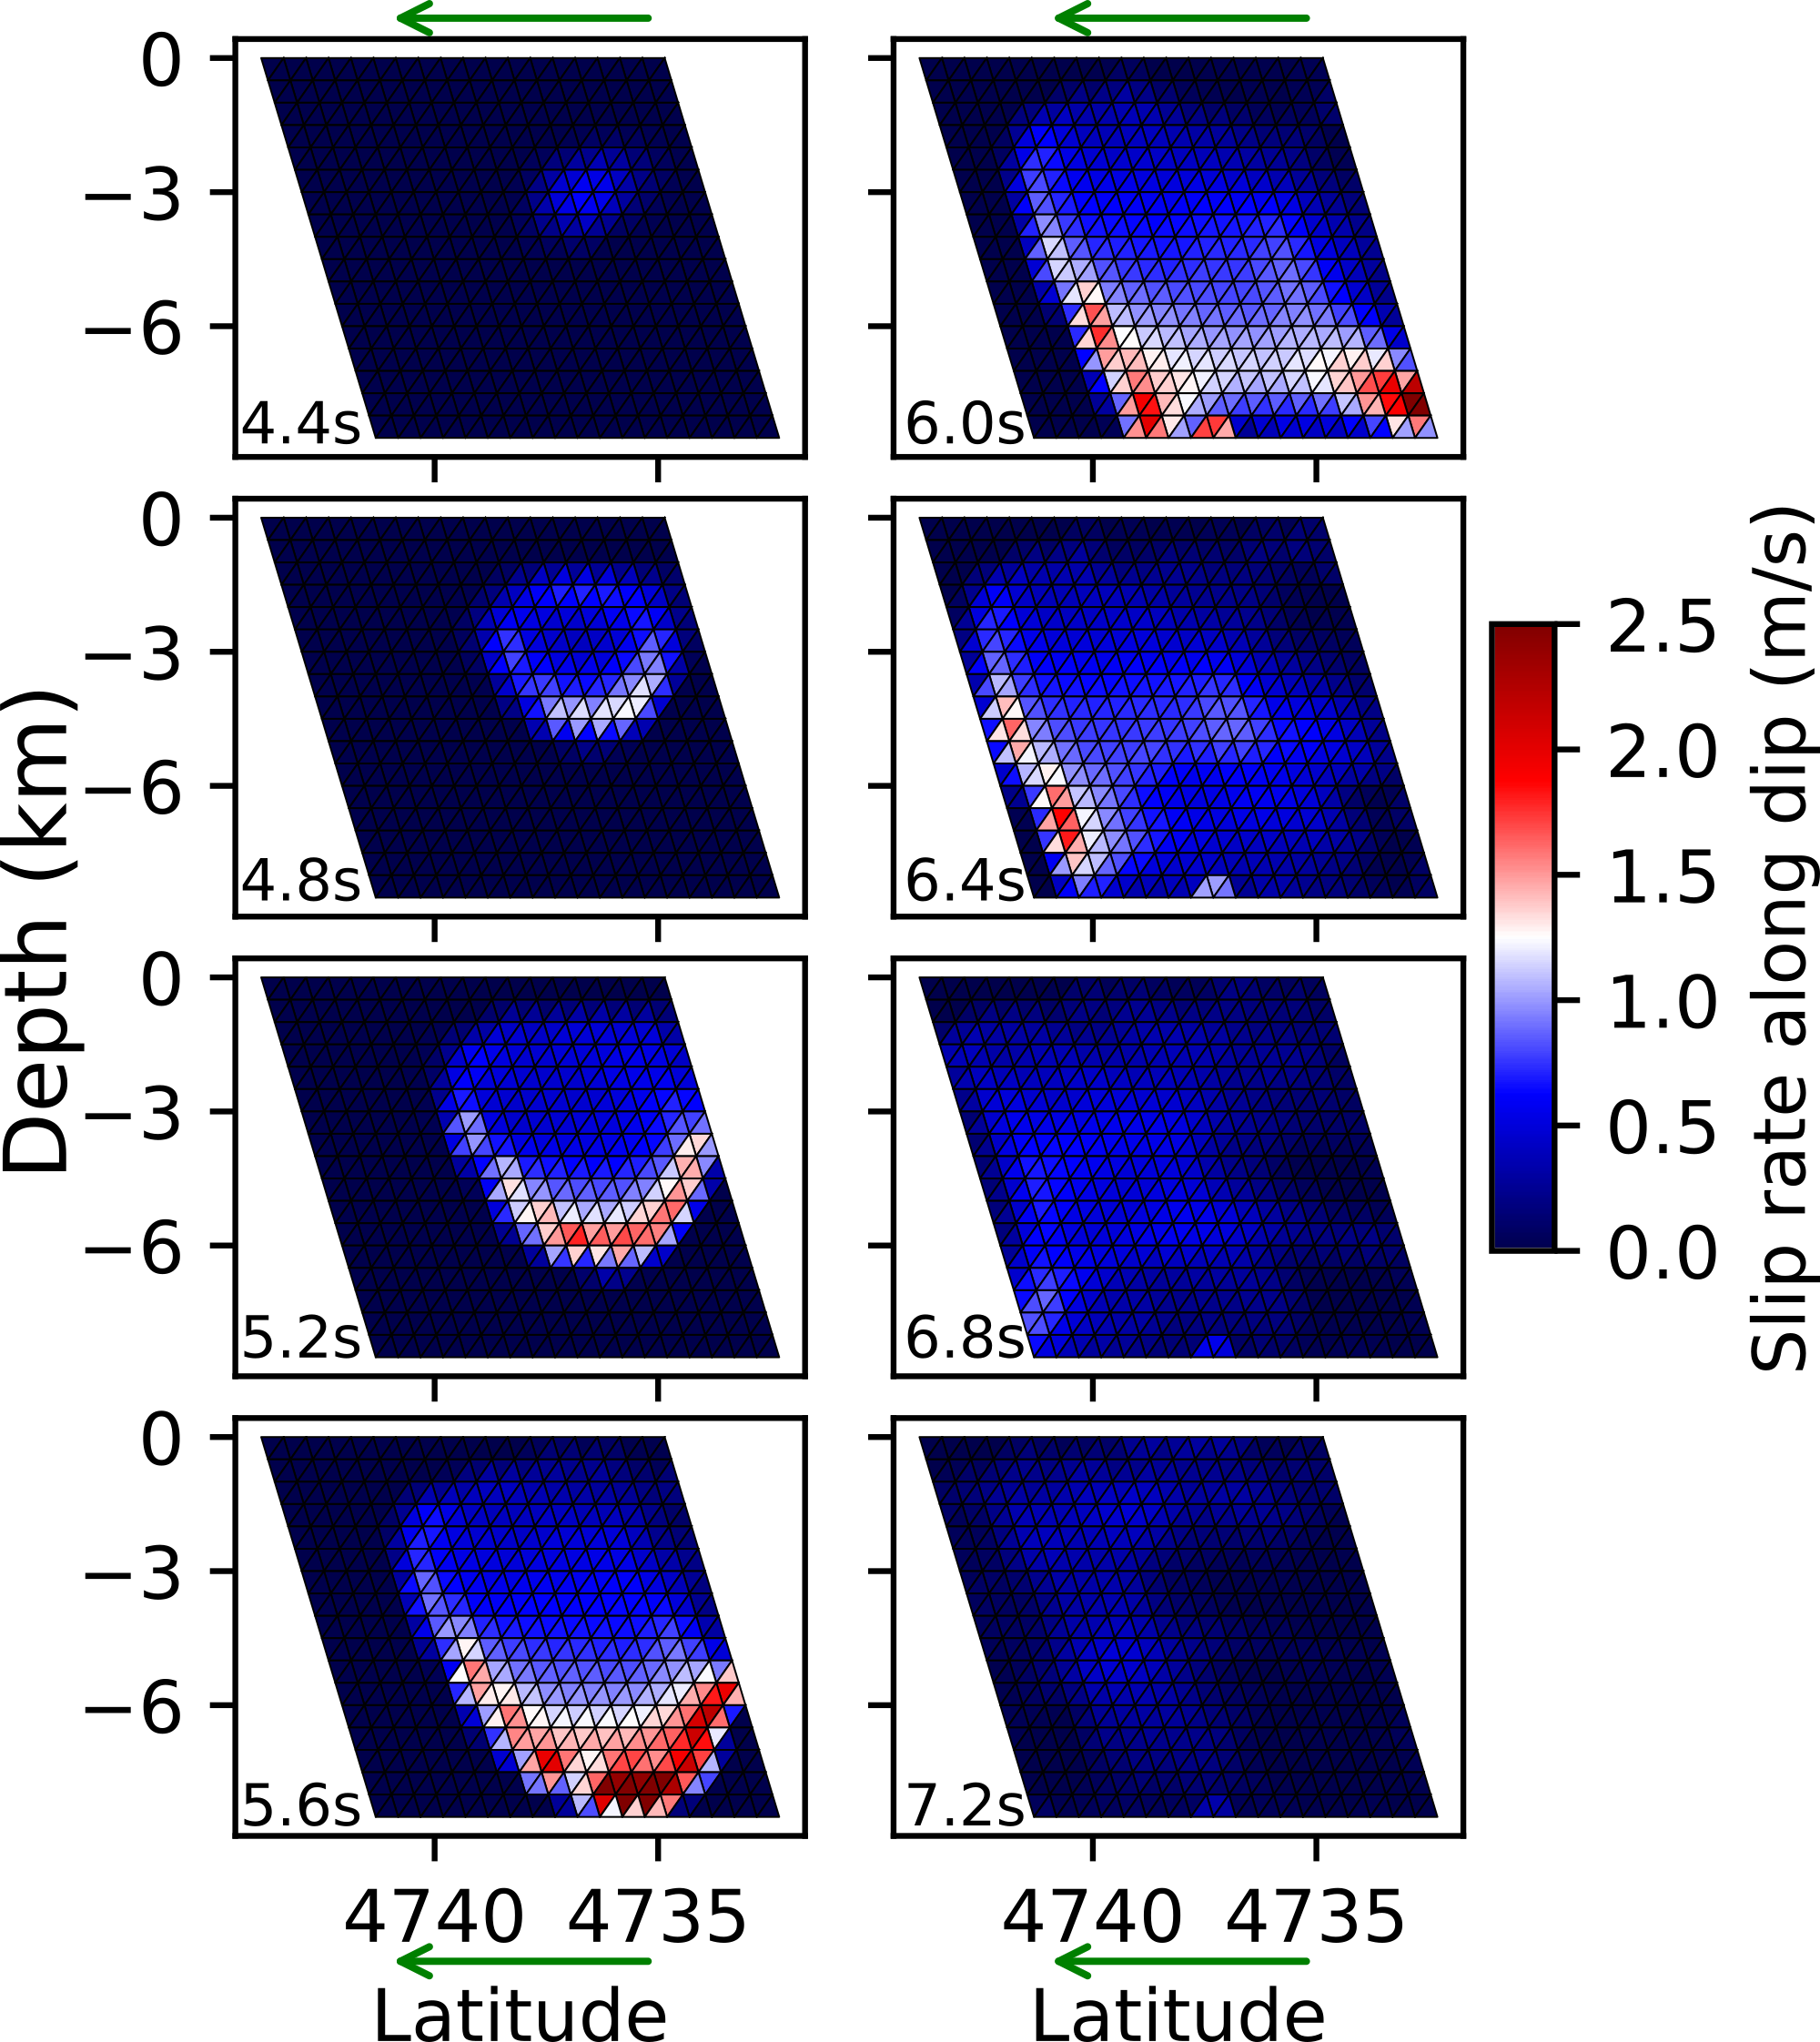
\includegraphics[width=0.95\linewidth]{images/snaps_00080.png}
\vskip 0.45cm
\hrule height 0.05cm
\vskip 0.2cm
 \centering {\bf Fault fixed ($\mu_s=50.0$)} \\
 (static analysis) \vskip 0.2cm
 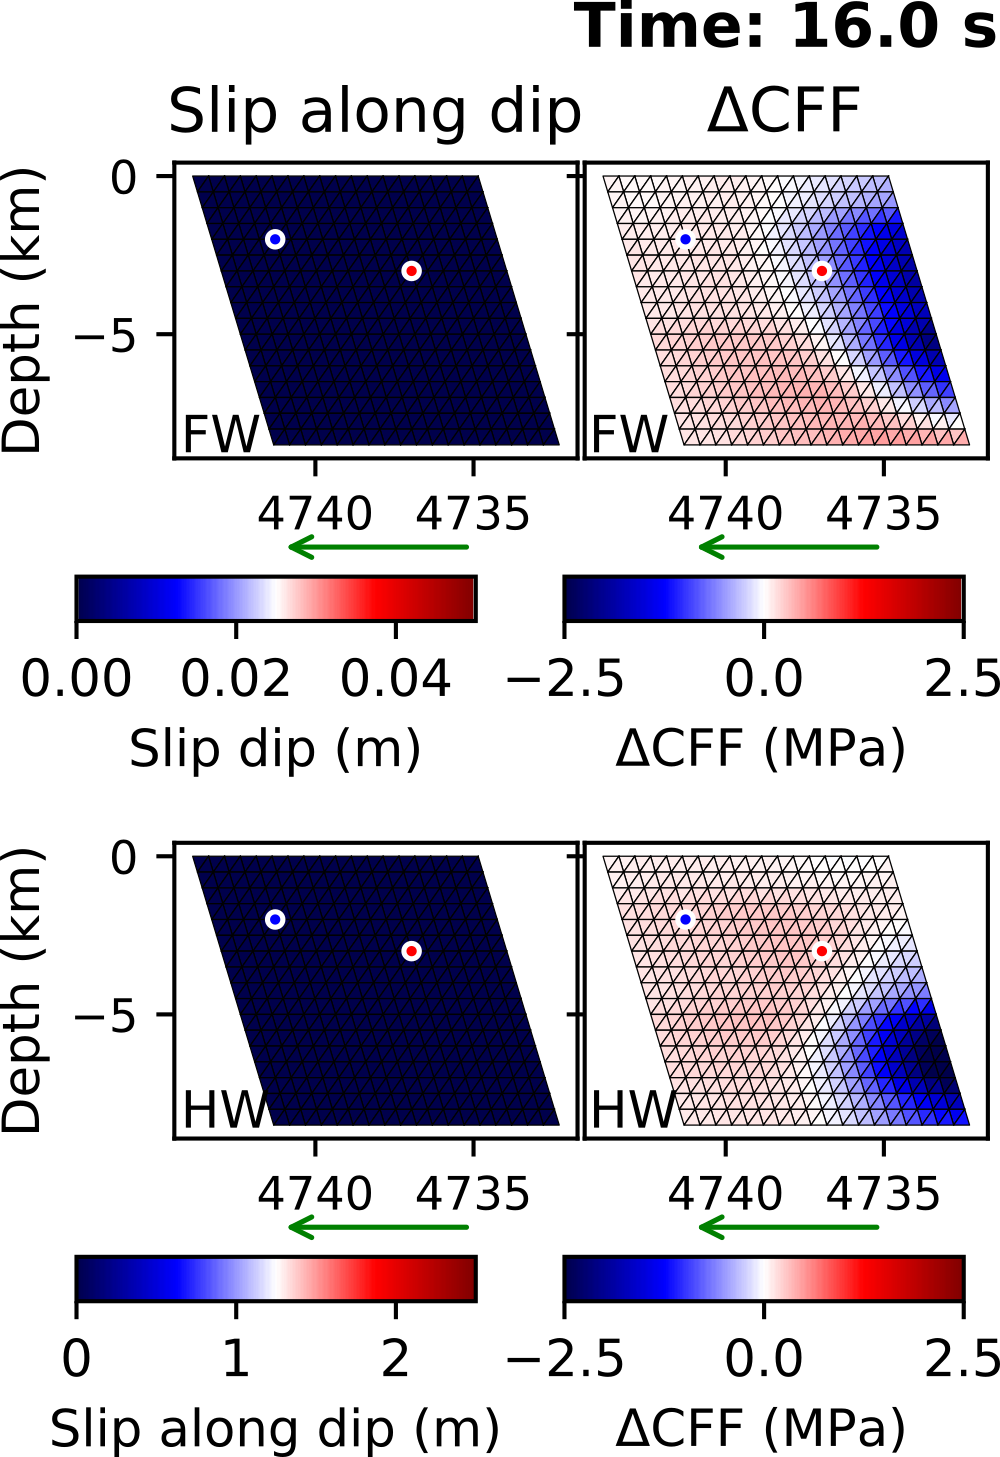
\includegraphics[width=0.87\linewidth]{images/horizontal_delta_00080_fix_1.png}
\vskip 0.2cm
\vskip 0.2cm
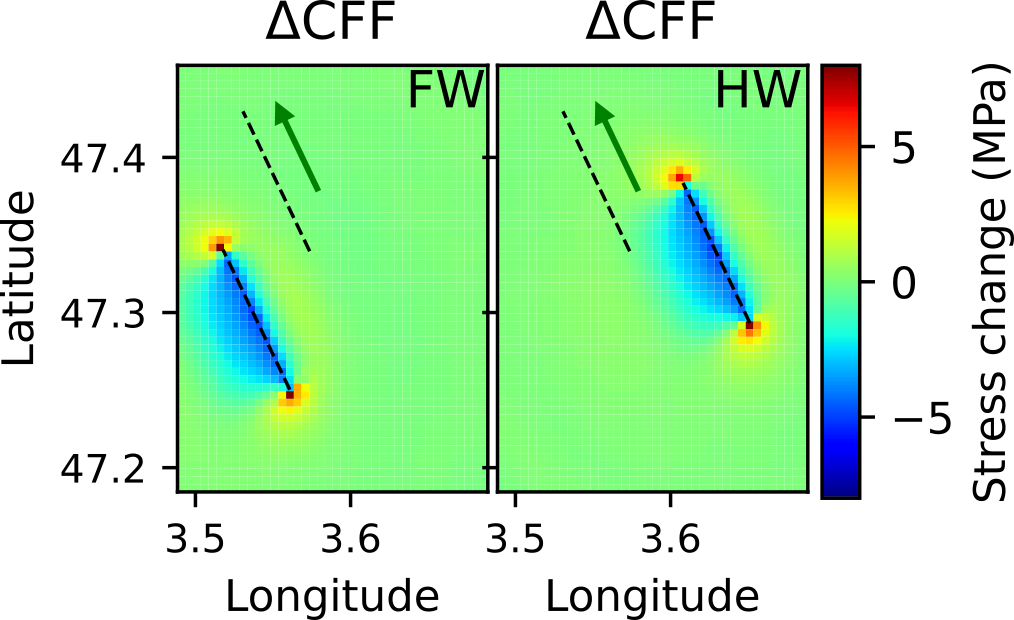
\includegraphics[width=0.87\linewidth]{images/horizontal_delta_00080_fix_2.png} \\
\vskip 0.2cm
\vskip 0.2cm
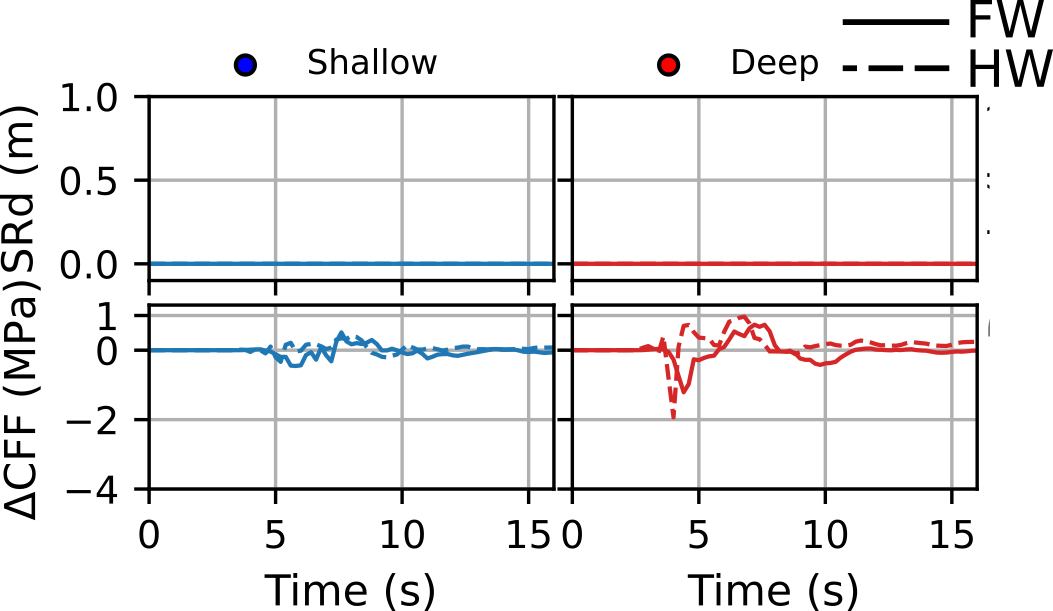
\includegraphics[width=0.87\linewidth]{images/horizontal_delta_00080_fix_3.png} 
\end{minipage}
}

\headerbox{{\bf 5.} Conclusion \& Discusion}{name=obs,column=1,row=2,span=1,below=snaps}{
\vskip -0.1cm
\ding{43} A static analysis seems insuficient to determine a \\
{\bf ``break-away"} behavior across step-over jumps.\\
\vskip -0.4cm
\ding{43} A maximum {\bf 5 km} step-over distance can still be \\
crossed and promote {\bf break-away ruptures} when \\
pre-stress levels are high enough ($S=0.1$) and no \\
obstacles (geometry, SHmax direction, friction pro-\\
perties, etc.) are present.\\
\vskip -0.4cm
\ding{43} {\bf Break-away} ruptures on the 2nd fault seem to\\
be triggered by two {\it S} waves arriving simultaneously \\
to the 2nd fault from the northern and bottom ends \\ of the 1st fault.\\
\vskip -0.4cm
\ding{43} A positive $\Delta$CFF area on the 2nd fault is insufi-\\
cient to determine if the rupture will be triggered.\\
\vskip -0.4cm
\ding{43} Triggered by coinciding arrival of several waves?
}


\headerbox{\,}{name=ref,column=2,row=2,span=1,above=bottom}{

\nocite{Improta_2019_AVN}
\nocite{Bernard_1989_IRPINIA}
\nocite{Valoroso_2013_AQUILA}
\nocite{Uphoff_2017_ESM}
\vskip -0.7cm
    \setlength{\bibsep}{5pt plus 0.2ex} {\tiny
    \begin{spacing}{1.2}
    \bibliography{biblio/bibtemp} 
    \end{spacing}
    }							
    \bibliographystyle{apalike}    
}

\end{poster}
\end{document}

 









%\headerbox{{\bf 5.} Results}{name=results,column=1,row=2,span=1,above=bottom}{

%}




